
\begin{comment}
Template vir elke funksie
        \paragraph{}
			\begin{description}
			    \item{\textbf{Priority}:} %watter prioriteit dit het: Critical, Important of Nic-to-have
			    \item{\textbf{Service Contract}:}% Wat dit doen
			    \item{\textbf{Pre-conditions}:}%wat moet waar wees voor die funksie sy ding kan doen
    			    \begin{itemize}
    			        \item %precondition 1
    			        \item %precondition 2
    			    \end{itemize}
			    \item{\textbf{Post-conditions}:} % wat moet waar wees na die funksie sy ding gedoen het
    			    \begin{itemize}
    			    \item %post condition 1
    			    \item %post condition2
    			    \end{itemize}
			\end{description}
\end{comment}




\subsection{Malware Server}

    \subsubsection{Scope}
	With the server the user will be able to target a specific android device to start recording and streaming the data back to the server.
		\begin{figure}[H]
 			 \centering
			  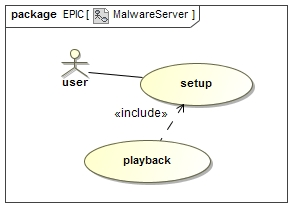
\includegraphics[width=12cm]{MalwareServerUseCase}
		 	 \caption{A Use Case Diagram of the Malware Server}
		\end{figure}
	
	
	\subsubsection{Functionality}
   
        \paragraph{sendStartRequest}
			\begin{description}
			    \item{\textbf{Priority}:} Critical%watter prioriteit dit het: Critical, Important of Nic-to-have
			    \item{\textbf{Service Contract}:}
			    This service will send a request to a specific mobile device that has the malware application installed to start a live stream.
			    \item{\textbf{Pre-conditions}:}%wat moet waar wees voor die funksie sy ding kan doen
    			    \begin{itemize}
    			        \item The malware application has created a connection with the server.
    			        \item The setup modules has been initialised.
    			    \end{itemize}
			    \item{\textbf{Post-conditions}:} % wat moet waar wees na die funksie sy ding gedoen het
    			    \begin{itemize}
    			    \item Receive the live stream.
    			    \end{itemize}
			\end{description}

    
         \paragraph{sendStopRequest}
			\begin{description}
			    \item{\textbf{Priority}:} Critical%watter prioriteit dit het: Critical, Important of Nic-to-have
			    \item{\textbf{Service Contract}:} This service sends a request to the malware application on a specified device to stop the live streaming.% Wat dit doen
			    \item{\textbf{Pre-conditions}:}%wat moet waar wees voor die funksie sy ding kan doen
    			    \begin{itemize}
    			        \item The server must be busy recording a live steam.
    			        \item The setup modules has been initialised.
    			    \end{itemize}
			    \item{\textbf{Post-conditions}:} % wat moet waar wees na die funksie sy ding gedoen het
    			    \begin{itemize}
    			    \item A stop request was sent to the malware application on the remote mobile device.
    			    \item A local recording of the live stream was stored on the server.
    			    \end{itemize}
			\end{description}
		
		
		\paragraph{playback}
			\begin{description}
			    \item{\textbf{Priority}:} Critical%watter prioriteit dit het: Critical, Important of Nic-to-have
			    \item{\textbf{Service Contract}:} The recorded stream is played back to the user over the speakers.% Wat dit doen
			    \item{\textbf{Pre-conditions}:}%wat moet waar wees voor die funksie sy ding kan doen
    			    \begin{itemize}
    			        \item The server must be busy recording a live steam.
    			        \item The setup modules has been initialised.
    			    \end{itemize}
			    \item{\textbf{Post-conditions}:} % wat moet waar wees na die funksie sy ding gedoen het
    			    \begin{itemize}
    			    \item A stop request was sent to the malware application on a specified device.
    			    \item The RecordingThread thread was closed.
    			    \end{itemize}
			\end{description}
	
	
        \paragraph{setup}
			\begin{description}
			    \item{\textbf{Priority}:}Critical %watter prioriteit dit het: Critical, Important of Nic-to-have
			    \item{\textbf{Service Contract}:} Initialise the audio recording modules. Creates a recording thread to handle the live stream and to create a local copy of the stream.% Wat dit doen
			    \item{\textbf{Pre-conditions}:}%wat moet waar wees voor die funksie sy ding kan doen
    			    \begin{itemize}
    			        \item The malware application has created a connection with the server.
    			    \end{itemize}
			    \item{\textbf{Post-conditions}:} % wat moet waar wees na die funksie sy ding gedoen het
    			    \begin{itemize}
    			    \item A RecordingThread thread was created.
    			    \item Playback has been initialised.
    			    \end{itemize}
			\end{description}
			
			
        \paragraph{selectPhone}
			\begin{description}
			    \item{\textbf{Priority}:} Critical%watter prioriteit dit het: Critical, Important of Nic-to-have
			    \item{\textbf{Service Contract}:} Creates a list for selection of a device to stream and record from.% Wat dit doen
			    \item{\textbf{Pre-conditions}:}%wat moet waar wees voor die funksie sy ding kan doen
    			    \begin{itemize}
    			        \item The malware application has created a connection with the server.
    			        \item A ClientThreads thread exists which handles the connections
    			    \end{itemize}
			    \item{\textbf{Post-conditions}:} % wat moet waar wees na die funksie sy ding gedoen het
    			    \begin{itemize}
    			    \item The setup modules has been initialised.
    			    \item A RecordingThread thread was created.
    			    \end{itemize}
			\end{description}
	
	
        \paragraph{createConnection}
			\begin{description}
			    \item{\textbf{Priority}:} Critical%watter prioriteit dit het: Critical, Important of Nic-to-have
			    \item{\textbf{Service Contract}:} Provides the means to create a list of devices to connect to and to create the connection to a mobile device running the malware application.% Wat dit doen
			    \item{\textbf{Pre-conditions}:}%wat moet waar wees voor die funksie sy ding kan doen
    			    \begin{itemize}
    			        \item Ports 4545 and 8080 must be allowed in the firewall
    			        \item The server is not currently receiving a live stream.
    			    \end{itemize}
			    \item{\textbf{Post-conditions}:} % wat moet waar wees na die funksie sy ding gedoen het
    			    \begin{itemize}
    			    \item A ClientThreads thread was created. 
    			    \item The connection to a mobile device running the malware application was successful.
    			    \end{itemize}
			\end{description}
	
	
        \paragraph{rawToWav}
			\begin{description}
			    \item{\textbf{Priority}:} Important%watter prioriteit dit het: Critical, Important of Nic-to-have
			    \item{\textbf{Service Contract}:} Converts the RAW audio file to a WAVE file. 	% Wat dit doen
			    \item{\textbf{Pre-conditions}:}%wat moet waar wees voor die funksie sy ding kan doen
    			    \begin{itemize}
    			        \item A stop request was sent to the malware application on the remote mobile device.
    			        \item The RecordingThread thread was closed.
    			    \end{itemize}
			    \item{\textbf{Post-conditions}:} % wat moet waar wees na die funksie sy ding gedoen het
    			    \begin{itemize}
    			    \item The RAW audio file was removed
    			    \end{itemize}
			\end{description} 
	
	
        \paragraph{copyWaveFile}
			\begin{description}
			    \item{\textbf{Priority}:} Important%watter prioriteit dit het: Critical, Important of Nic-to-have
			    \item{\textbf{Service Contract}:}Takes the WAVE file and adds the required header to the file to enable correct playback.% Wat dit doen
			    \item{\textbf{Pre-conditions}:}%wat moet waar wees voor die funksie sy ding kan doen
    			    \begin{itemize}
    			        \item The RAW audio file was converted to a WAVE file
    			        \item The RAW audio file was removed
    			    \end{itemize}
			    \item{\textbf{Post-conditions}:} % wat moet waar wees na die funksie sy ding gedoen het
    			    \begin{itemize}
    			    \item The required header values was added to the wave file. 
    			    \end{itemize}
			\end{description}
	
        \paragraph{MainMenu}
			\begin{description}
			    \item{\textbf{Priority}:} Nice to have%watter prioriteit dit het: Critical, Important of Nic-to-have
			    \item{\textbf{Service Contract}:} Creates a user friendly interface for using the server.% Wat dit doen
			    \item{\textbf{Pre-conditions}:}%wat moet waar wees voor die funksie sy ding kan doen
    			    \begin{itemize}
    			        \item No previous interface exists.
    			    \end{itemize}
			    \item{\textbf{Post-conditions}:} % wat moet waar wees na die funksie sy ding gedoen het
    			    \begin{itemize}
    			    \item Interface listeners are active
    			    \item Main menu is visible.
    			    \end{itemize}
			\end{description}
	   	
				